\newpage

\begin{figure*}[t]
\centering
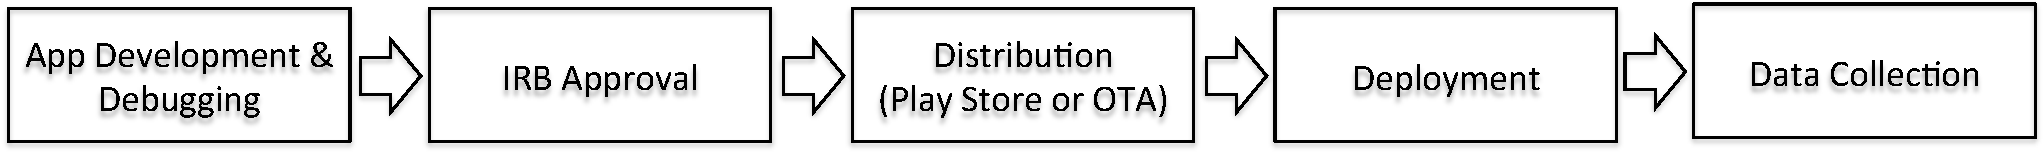
\includegraphics[width=0.9\textwidth]{experiment-life-cycle.pdf}
\caption{Expected Life Cycle of a \PhoneLab{} Experiment}
\label{fig:experiment-life-cycle}
\end{figure*}

\section{Experiment Case Study}
\label{sec-experiment}

We have conducted a measurement study to demonstrate the power of \PhoneLab{};
we have developed a logging tool, deployed it on 88 participant phones, and
collected data for 21 days. As mentioned in Section~\ref{sec:comparison}, 
a measurement study is an ideal candidate to demonstrate the power of
\PhoneLab{} because it requires a combination of many features of \PhoneLab{},
e.g., scale, realism, timeliness, and participant control. In a sense, a
measurement study ``stress tests'' the power of \PhoneLab{}.

We first give a look into how an experiment can be performed on \PhoneLab{} by
describing the expected life cycle of an experiment.
Figure~\ref{fig:experiment-life-cycle} overviews an expected life cycle of an
experiment. We then report how our own experiment proceeded for each step of the
life cycle.

\subsection{Experiment Life Cycle}

A typical \PhoneLab{} experiment will proceed in the following five steps.

{\bf App Development and Debugging:} The first step is (obviously) application
development and debugging. Since we do not consider \PhoneLab{} as a debugging
facility, we expect \PhoneLab{} users to do a thorough job of local testing and
consider their applications as ``final products.'' Distribution via the Play
Store will help in this regard because it imparts the sense that an application
developed for \PhoneLab{} is a product released to the public.

Thorough local testing is important for both \PhoneLab{} participants and users.
For participants, buggy or power-hungry software will irritate them and disrupt
their normal daily phone usage. This behavioral change will affect the users as
well because it might affect the quality of the results they get; participants'
behaviors might deviate from their normal usage patterns. In addition, since we
do not force our participants to participate in any particular experiment, buggy
or power-hungry software can reduce the chance of participation.

{\bf IRB Approval:} Perhaps the biggest difference between \PhoneLab{} and other
existing testbeds is the requirement for IRB approval. In existing testbeds,
users mainly interact with machines, not humans, so there is no need for IRB
approval. In contrast, \PhoneLab{} users (or more precisely, their experimental
software) need to interact with humans either directly via the phone UI or
indirectly as a background service. This inevitably bears the question of
privacy and protection. In fact, protecting our participants is one of our
primary operational objectives because participants are a vital part of
\PhoneLab{}.

This IRB approval is a requirement for every experiment. We recognize that some
experiments do not need to get any approval, in which case we require a letter
stating the irrelevance. The IRB approval should be done per experiment by the
experimenters through their own institution's IRB. SUNY Buffalo's IRB does not
get involved in this process. Given the popularity of smartphone research
evaluation with real devices and users, we expect that many researchers in the
mobile systems community are already familiar with their own IRB process.

{\bf Distribution:} Our distribution channels are different for
application-level experiments and platform-level experiments. For
application-level experiments, we leverage the Play Store as our distribution
channel. In the early design stages, we explored an option of providing our own
distribution channel even for application-level experiments. However, we
realized later that Play Store provides all the features we need: a description
page, an automatic update mechanism, permission display, download statistics,
etc. For platform-level experiments, we will use our own OTA (Over-The-Air)
distribution mechanism currently in development.

{\bf Deployment:} Deployment for an experiment is done by each participant
individually. For an application-level experiment, each participant downloads
the application for the experiment from the Play Store. We have instructed our
participants to examine each description and permission requested for every
experiment they participate. This will continue in the future as well. As
mentioned before, we do not force any participant to participate in any
particular experiment. If they feel uncomfortable about the permissions
requested and information collected from their phones, they can either choose to
not participate or stop participating in the middle of the experiment. This is
also a typical requirement from IRB for any experiment. For a platform-level
experiment, we notify every participant for the availability of a new
experimental platform image, kernel image, or both. When a participant agrees to
participate, the OTA process begins and re-flashes the phone.

{\bf Data Collection:} \PhoneLab{} users are encouraged to leverage the data
logging and collection mechanism we provide using the standard Android logging
API (\texttt{android.util.Log}). This mechanism collects logs from every phone
when the phone is being plugged in and connected to a network. If for some
reason a \PhoneLab{} user find our data collection inadequate, the user can
incorporate a custom data logging and collection.

\subsection{Our Experiment}

{\bf App Development and Debugging:} Tool description. What we collect and where
we get it. Say that we're doing something similar to PowerTutor for battery
using Java reflection for fuelgauge. Comprehensive collection of information
(list them). 15 min interval to reduce power consumption. Power was the main
concern for our development.

{\bf IRB Approval and Distribution:} Started when and finished when. Delay is
mainly because of us. IRB side review itself took (how long). We uploaded our
first version on (date).

{\bf Deployment:} How long did it take to reach 88? Say that this in and of
itself is an experiment because we only sent out one mass email annoucing the
availability of the play store app.

{\bf Data Collection:} How much did we generate?
